\subsection{Troubleshooting Guide}

\newline
\begin{itemize}
\item Why~don’t~any~labs~appear~on~the~OpenScienceLab~home~page?
\item Why~did~the~kernel~die~while~running~a~notebook?
\item I~successfully~ran~a~notebook~earlier~on~the~same~data~but~now~it~is~killing~the~kernel.
\item I~receive~a~Kernel~not~found~message~when~I~open~a~notebook.
\item My~notebook~won’t~open,~opens~slowly,~or~won’t~save.
\item I~am~receiving~a~No~space~left~on~device~error.
\item My~server~won’t~start~and~I~cannot~access~OpenSARlab.
\item The~edits~I~made~to~an~ASF~notebook~have~disappeared~since~the~last~time~I~used~OpenSARlab.
\item One~of~my~notebooks~looks~like~it~has~a~mix~of~code~from~various~versions~of~the~notebook.
\item I~am~having~trouble~setting~up~a~web~server~and~developing~my~web~app~in~OpenSARlab.
\item A~notebook~won’t~load.~A~new~browser~tab~opens~and~shows~the~JupyterHub~header,~but~no~notebook~appears.
\item My~issue~is~not~on~this~list
\end{itemize}

\subsubsection{Why don't any labs appear on the OpenScienceLab home page?}\label{Why-dont-any-labs-appear-on-the-OpenScienceLab-home-page}

You most likely have not yet configured Multi-Factor Authentication (MFA). While
any user can log in without MFA, until a user has configured their MFA device,
they will be unable to access any OpenScienceLab resources.

See \href{/mfa}{Configuring Multi-Factor Authentication} for more information and
a detailed walkthrough.

\subsubsection{Why did the kernel die while running a notebook?}\label{Why-did-the-kernel-die-while-running-a-notebook}

\begin{figure}[!htbp]
\centering
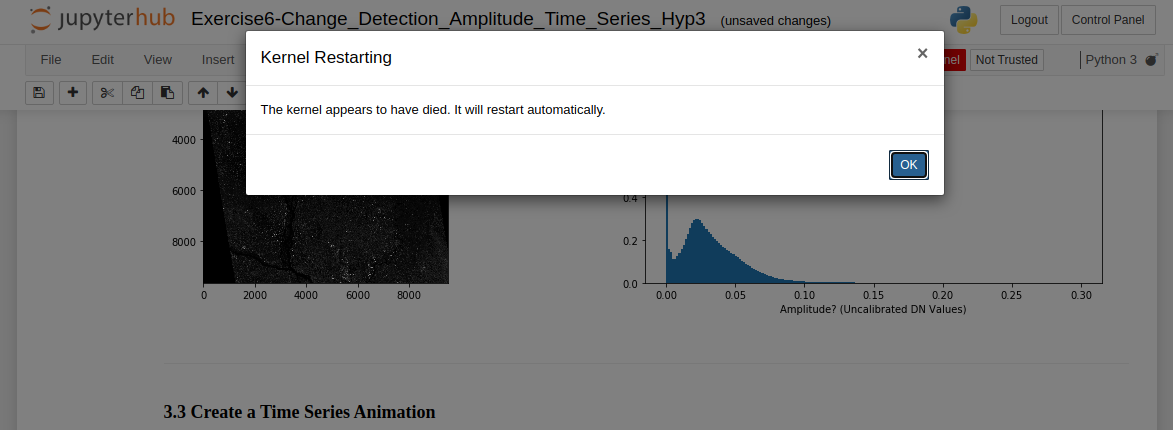
\includegraphics[width=0.7\linewidth]{files/kernel_death-d28efc694e1f525cac874ac5cff0e697.png}
\caption*{The message that appears when a notebook kernel dies}
\end{figure}

\begin{itemize}
\item The kernel will die if you run out of available memory to complete a running process. This occurs frequently when running a time-series or change detection algorithm on data stack that is either too deep or covers too large of an area-of-interest (AOI) for OpenSARLab to handle.


\item Try running the notebook on some combination of a shallower data stack and/or a smaller AOI. This may take some experimentation because memory is shared among users, \textit{i.e.} amount of available memory fluctuates.


\item To work with a deep stack covering an extensive AOI, you may need to tile up your data for the analysis and mosaic them later.
\end{itemize}

\textit{Summary:} If you are running a resource hungry program, your kernel might die. Try subsetting your data, processing it in batches, and mosaicing your results.


\bigskip
\centerline{\rule{13cm}{0.4pt}}
\bigskip

\subsubsection{I successfully ran a notebook earlier on the same data but now it is killing the kernel.}\label{I-successfully-ran-a-notebook-earlier-on-the-same-data-but-now-it-is-killing-the-kernel}

\begin{itemize}
\item OpenSARLab EC2 instances are shared among 1{\textasciitilde}3 users. The memory available to each user depends on overall activity on the EC2. It is likely that there was enough memory available for your process before, but not enough memory during later attempt(s). More details on the OpenSARLab user environment can be found \href{OpenSARLab\_environment.md}{here}.
\end{itemize}


\bigskip
\centerline{\rule{13cm}{0.4pt}}
\bigskip

\subsubsection{I receive a \texttt{Kernel not found} message when I open a notebook.}\label{I-receive-a-Kernel-not-found-message-when-I-open-a-notebook}

\begin{figure}[!htbp]
\centering
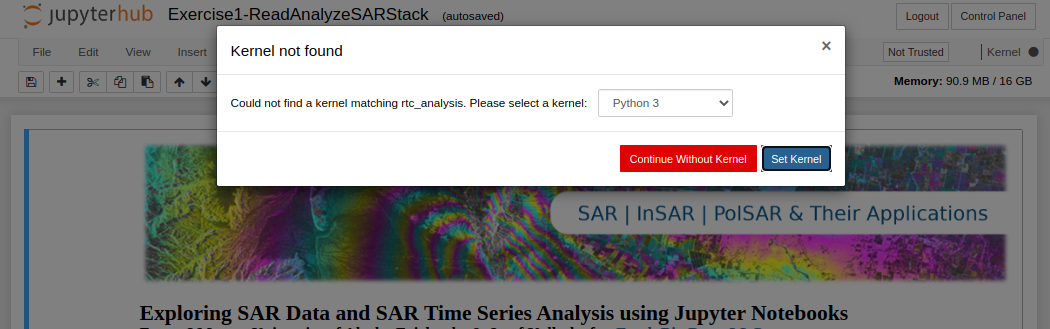
\includegraphics[width=0.7\linewidth]{files/kernel_not_found-b803e941d26eecaaafd4dc583a6ba310.png}
\caption*{The message that appears when an expected notebook kernel cannot be found}
\end{figure}

\begin{itemize}
\item You either have:

\begin{itemize}
\item Not created the required conda environment yet
\item A mix-up between the environment name and prefix
\end{itemize}


\item If you think you already installed the environment, select it from the pull-down menu that appears and click the \texttt{Set Kernel} button.


\item If you have not created the environment yet:

\begin{itemize}
\item In OpenSARLab, you can find a selection of environments and a notebook to build them here: \href{https://opensciencelab.asf.alaska.edu/lab/smce-prod-opensarlab/hub/user-redirect/lab/tree/conda\_environments/Create\_OSL\_Conda\_Environments.ipynb}{\texttt{/home/jovyan/conda\_environments/Create\_OSL\_Conda\_Environments.ipynb}}
\item If you are working in an ASF-supplied Jupyter Book, it should include a notebook to build the required environment/s
\end{itemize}
\end{itemize}


\bigskip
\centerline{\rule{13cm}{0.4pt}}
\bigskip

\subsubsection{My notebook won't open, opens slowly, or won't save.}\label{My-notebook-wont-open-opens-slowly-or-wont-save}

\begin{itemize}
\item These are all signs that the notebook contains a lot of output and is too large to easily open or save over the internet in OpenSARLab.\begin{itemize}
\item If the notebook won't open or opens very slowly, remove its output by running the following command from a terminal:\begin{itemize}
\item \texttt{jupyter nbconvert --clear-output --inplace my\_notebook.ipynb}
\end{itemize}


\item If the notebook is open and you can't save it, try clearing its output first.
\end{itemize}
\end{itemize}

\begin{figure}[!htbp]
\centering
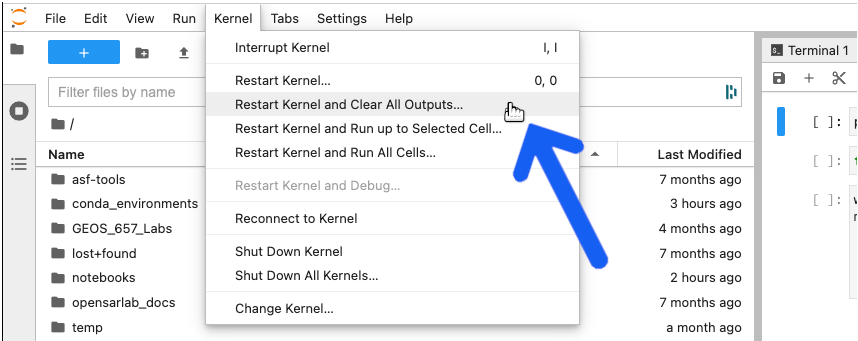
\includegraphics[width=0.7\linewidth]{files/restart_clear_all_jl-69996a882d58b2b807efb0170b60c542.png}
\caption*{Select \texttt{Restart Kernel and Clear All Outputs} from the \texttt{Kernel} menu and try saving it again.}
\end{figure}


\bigskip
\centerline{\rule{13cm}{0.4pt}}
\bigskip

\subsubsection{I am receiving a \texttt{No space left on device} error.}\label{I-am-receiving-a-No-space-left-on-device-error}

OpenSARLab users have access to a finite amount of storage space (\href{OpenSARlab\_environment.md}{details here}).

\textbf{It is up to users to manage their storage}.

\begin{itemize}
\item If you receive a storage space warning while logged into OpenSARlab, it is highly recommended to free up your space immediately by deleting unnecessary files. If your server shuts down without any available space, it will not have enough space on your volume to restart again and you will be locked out of your account.


\item If you do get locked out from your account, contact an \href{mailto:uaf-jupyterhub-asf@alaska.edu}{OpenSARlab administrator} for help.
\end{itemize}


\bigskip
\centerline{\rule{13cm}{0.4pt}}
\bigskip

\subsubsection{My server won't start and I cannot access OpenSARlab.}\label{My-server-wont-start-and-I-cannot-access-OpenSARlab}

This issue is typically due either to an unexpected behavior of \href{https://jupyterhub.github.io/nbgitpuller/}{nbgitpuller} or to having used up all space on your storage volume.

Please contact an \href{mailto:uaf-jupyterhub-asf@alaska.edu}{OpenSARlab Administrator} for help.


\bigskip
\centerline{\rule{13cm}{0.4pt}}
\bigskip

\subsubsection{The edits I made to an ASF notebook have disappeared since the last time I used OpenSARlab.}\label{The-edits-I-made-to-an-ASF-notebook-have-disappeared-since-the-last-time-I-used-OpenSARlab}

\begin{itemize}
\item When your OpenSARlab server starts up, \texttt{nbgitpuller} runs and pulls in any updates made to the \href{https://github.com/asfadmin/asf-jupyter-notebooks}{asf-jupyter-notebooks} and other Jupyter Book GitHub repositories provided in OpenSARLab. If a change has been made to a notebook by both the user and the author, both changes will be saved. The author's updated version will retain its original name while the user's version will have a timestamp appended to its name.
\end{itemize}

\begin{framed}
\textbf{Example file naming format for updated notebooks synched with \texttt{nbgitpuller}}\\
Notebook containing new updates: \texttt{sample\_notebook.ipynb}

Notebook previously edited by user, now with a timestamp appended to the name: \texttt{sample\_notebook\_20240616165846.ipynb}
\end{framed}

\begin{itemize}
\item If you think your notebook is missing, it is likely in its original location with a recent timestamp appended to its name.
\end{itemize}


\bigskip
\centerline{\rule{13cm}{0.4pt}}
\bigskip

\subsubsection{One of my notebooks looks like it has a mix of code from various versions of the notebook.}\label{One-of-my-notebooks-looks-like-it-has-a-mix-of-code-from-various-versions-of-the-notebook}

\begin{itemize}
\item We have seen this happen occasionally and it is caused by \href{https://jupyterhub.github.io/nbgitpuller/}{nbgitpuller}. The best option is to delete the notebook and \href{restarting\_server\_and\_kernel.md}{restart your OpenSARlab server}. The notebook will be replaced with a fresh copy from its nbgitpuller-managed repository.
\end{itemize}


\bigskip
\centerline{\rule{13cm}{0.4pt}}
\bigskip

\subsubsection{I am having trouble setting up a web server and developing my web app in OpenSARlab.}\label{I-am-having-trouble-setting-up-a-web-server-and-developing-my-web-app-in-OpenSARlab}

\begin{itemize}
\item This cannot be done in OpenSARlab. You will need to do this elsewhere.
\end{itemize}


\bigskip
\centerline{\rule{13cm}{0.4pt}}
\bigskip

\subsubsection{A notebook won't load. A new browser tab opens and shows the JupyterHub header, but no notebook appears.}\label{A-notebook-wont-load-A-new-browser-tab-opens-and-shows-the-JupyterHub-header-but-no-notebook-appears}

\begin{itemize}
\item This is due to slow loading time caused by a large notebook.


\item If you run a notebook and close it without clearing all output from the code cells, the file size will increase. This may cause it to load very slowly, depending on a user's network bandwidth.

\begin{itemize}
\item \textit{A 40KB notebook can grow to over 60MB if you don't clear its output.}
\end{itemize}


\item Try clearing the notebook's output before opening it by running the following command in the terminal:

\begin{itemize}
\item \texttt{jupyter nbconvert --clear-output --inplace my\_notebook.ipynb}
\end{itemize}
\end{itemize}


\bigskip
\centerline{\rule{13cm}{0.4pt}}
\bigskip

\subsubsection{My issue is not on this list}\label{My-issue-is-not-on-this-list}

\begin{itemize}
\item Please contact an \href{mailto:uaf-jupyterhub-asf@alaska.edu}{OpenSARlab administrator} for help.
\end{itemize}

%  TODO: add documentation in regards to server timeouts